% =========================================================================== %
% Yes. This is a document.

\documentclass[
	english,
	aspectratio=169,
	table
]{beamer}

% =========================================================================== %
% Theme
\usepackage{scrlfile}
	\ReplacePackage{beamerthemeSHUR}{./sty/beamerthemeSHUR}
	\ReplacePackage{beamerinnerthemefancy}{./sty/beamerinnerthemefancy}
	\ReplacePackage{beamerouterthemedecolines}{./sty/beamerouterthemedecolines}
	\ReplacePackage{beamercolorthemechameleon}{./sty/beamercolorthemechameleon}

\usetheme[
	pageofpages=/,
	bullet=circle,
	titleline=true,
	alternativetitlepage=true,
	watermark="",
	watermarkheight=0px,
	watermarkheightmult=0
	]
{SHUR}

% =========================================================================== %
% the usual stuff

\usepackage[utf8]{inputenc}
\usepackage[T1]{fontenc}
\usepackage{babel}
\usepackage{lmodern}
\usepackage{microtype}
\usepackage{csquotes}

\usepackage{tabularx}
\usepackage{booktabs}
\usepackage{multirow}

\usepackage{color, colortbl}
\usepackage{xcolor}
	\definecolor{tabhighlight}{RGB}{230,240,255}

\usepackage{tabto}

\usepackage{minted}
	\usemintedstyle{friendly}

\usepackage{tikz}
	\usetikzlibrary{positioning}
	\usetikzlibrary{matrix}
	\usetikzlibrary{shapes.geometric}
	\usetikzlibrary{backgrounds}
	\usetikzlibrary{calc}
	\usetikzlibrary{decorations.pathreplacing}
	\tikzstyle{every picture}+=[remember picture] 
\usepackage{adjustbox}

\usepackage[most]{tcolorbox}
	\tcbsetforeverylayer
		{colback=cyan!10!white,
		 colframe=cyan!75!black,
		 arc=0pt,
		 outer arc=0pt
		}
	\newtcolorbox{codebox}[1][Code]
		{colback=black!5!white,
		 colframe=blue!40!black,
		 title=#1,
		 leftupper=6mm
		}
	\newtcolorbox{cmdbox}[1][Kommandozeilen-Befehl]
		{colback=black,
		 coltext=white,
		 fontupper=\ttfamily ,
		 colframe=blue!40!black,
		 title=#1,
		 outer arc=0pt
		}
	\newtcolorbox{warnbox}[1][Beachte]
		{colback=black!5!white,
		 colframe=red!40!black,
		 title=#1
		}
	\newtcolorbox{hintbox}[1][Tipp]
		{colback=black!5!white,
		 colframe=green!40!black,
		 title=#1
		}
	\newenvironment{itembox}
		{\begin{tcolorbox}\begin{itemize}}%
		{\end{itemize}\end{tcolorbox}}
	\newtcolorbox{doublebox}[1][.3]
		{righthand width=#1\linewidth,
		 sidebyside,
		 sidebyside gap=6mm,
		 sidebyside align=center,
		 lower separated=false}
	
%==============================================================================%
% GLOBAL MACROS

\newcommand*{\zB}{e.\,g. }
\newcommand*{\ie}{i.\,e. }

\newcommand{\Thus}{\ensuremath{\Rightarrow}}
\newcommand{\thus}{\ensuremath{\rightarrow}}

\newcommand*{\tabcrlf}{\\ \midrule}			% actually still allows for optional argument

\newcommand*{\inPy}[1]{\mintinline{python}{#1}}

% =========================================================================== %

\author{Stefan Hartinger}
\title{Programming in Python}
\subtitle{Part 1: Programming Environment and First Steps}
\institute{University Regensburg, Department of Theoretical Physics}
\date{Winter Term 2021/22}

% =========================================================================== %

\begin{document}
% =========================================================================== %

\begin{frame}[t,plain]
\titlepage
\end{frame}

% =========================================================================== %

\begin{frame}
%
\begin{center}

\includegraphics[width=.5\linewidth]{./gfx/intro}
\end{center}
%
\end{frame}

% =========================================================================== %

\begin{frame}{Our Mantra}
%
\begin{center}
\begin{Huge}
\emph{Computers are friggin stupid.}
\end{Huge}
\vspace{20pt}

As humans, we infer a ton of information implicitly and go thus through our lives. A computer cannot do that. Whenever there is even a quantum of ambiguity, computers will stop working. Anything happening automatically was consciously put there by a programmer (like us).
\vspace{10pt}

In this class, we'll learn how to analyze our own thought process and to formulate the results of this analysis in code.
\end{center}
%
\end{frame}

% =========================================================================== %

\begin{frame}{Programming in Python -- Historical Bla Bla}
%
\begin{itemize}
\item Since 2003: one of the top 10 languages in the TIBOE-Index (based on web-activity)
\item First published in 1991, continuously improved upon
\item Current stable release: Version 3.10 -- matter of this course
\item Major versions not 100\% compatible with one another, but the basic principles are the same (and can be transferred to other languages as well)
\item \enquote{Batteries included} -- many pre-built solutions to recurring problems
\item Script language -- optimized for fast development, good code readability and portability
\item Usually (much) slower in runtime than compiled languages -- factor 10
\end{itemize}
%
\end{frame}

% =========================================================================== %

\begin{frame}{Vocabulary: Interpreter}
%
\begin{minipage}{.49\linewidth}
\begin{itemize}
\item Code: (more or less) human language
\item Computer: executes enumerated \emph{elementary} commands, extremely small steps
\item Interpreter: Program that translates Code into machine language
\item Interpreters do that in \emph{real time}; compilers prepare a translation
\item Advantage: Interpreters handle machine-specific details; same code runs on (almost) all machines
\end{itemize}
\end{minipage}
%
%
\begin{minipage}[t]{.49\linewidth}
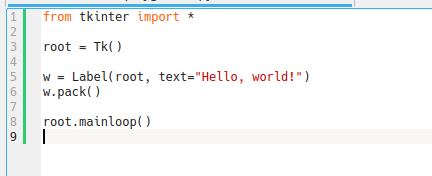
\includegraphics[width=\linewidth]{./gfx/TK-HelloWorld-Code}
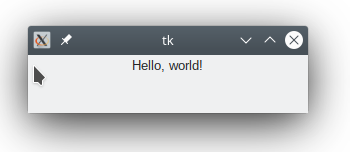
\includegraphics[width=\linewidth]{./gfx/TK-HelloWorld-Run}
\end{minipage}
%
\end{frame}

% =========================================================================== %

\begin{frame}{Vocabulary: Terminal}
%
\begin{columns}[T]
\column{.55\linewidth}
\begin{itemize}
\item Invoking the interpreter: (at least indirectly) via \emph{Terminal}
\item Human-Machine-Interface
\item Commands in human (or at least human-like) language
\item Until today: \emph{backend} for all computer systems
\item \emph{IDEs} (integrated development environment): more comfort, but no global design
\item Essentially: basic knowledge about terminals necessary whenever coding is to be done
\end{itemize}
%
\column{.4\linewidth}
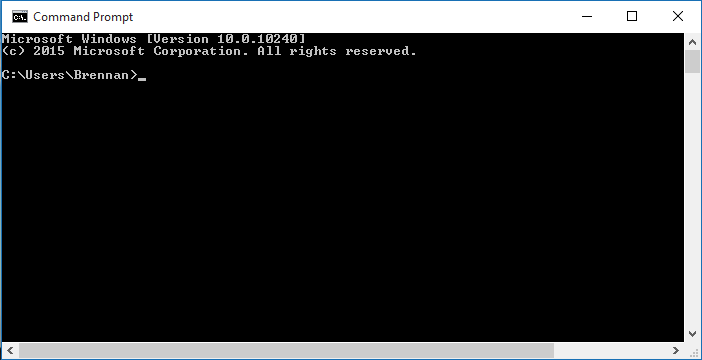
\includegraphics[width=\linewidth]{./gfx/cmd}
{\tiny Windows-Terminal: \texttt{cmd}}
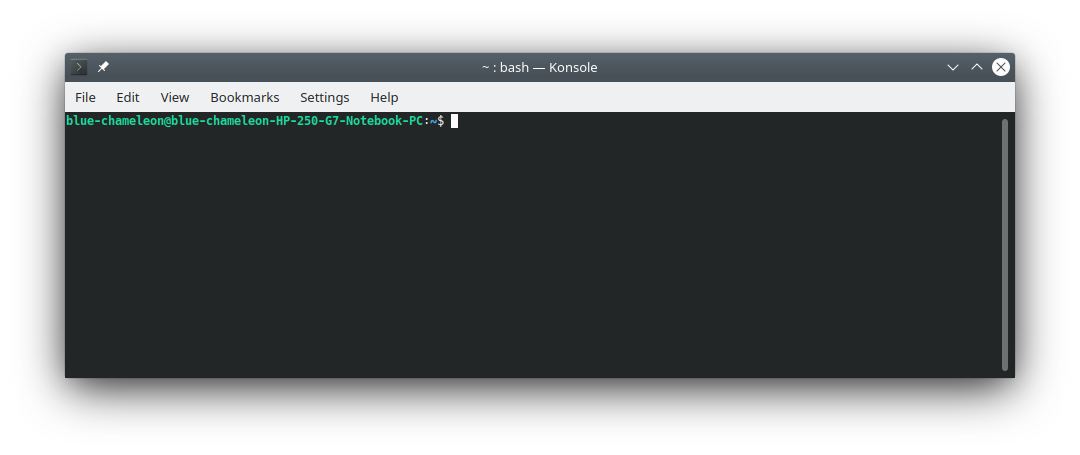
\includegraphics[width=\linewidth]{./gfx/bash}
{\tiny Linux-Terminal: \texttt{bash}}
\end{columns}
%
\end{frame}

% =========================================================================== %

\begin{frame}{Vocabulary: Current Working Directory (CWD)}
%
\begin{itemize}
\item Files on computers: structured into folders
\item Multiple files with same name in different folders possible
\item Computer needs to know \emph{unambiguously} which file should be accessed
\item Idea: \emph{Working Directory} -- \enquote{Where am I right now?}
\end{itemize}
%
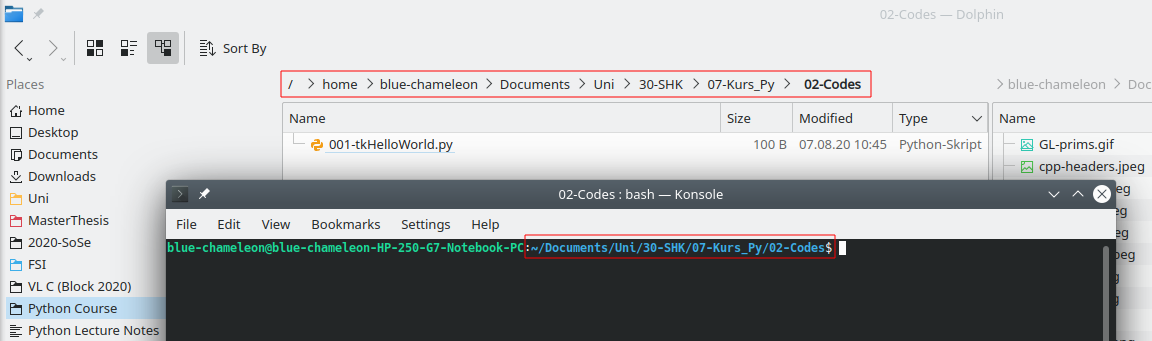
\includegraphics[width=\linewidth]{./gfx/paths}
%
\end{frame}

% =========================================================================== %

\begin{frame}{Launching Programs, Changing the CWD}
%
\begin{itemize}
\item Change directory: \texttt{cd}
	\begin{minipage}{\linewidth}
		\begin{minipage}{.49\linewidth}
		\begin{itemize}
		\item Either: multiple \enquote{steps} at once\\
			\texttt{cd directory/subdirectory}
		\end{itemize}
		\end{minipage}
		%
		\begin{minipage}{.49\linewidth}
		\begin{itemize}
		\item Or: multiple commands in sequence\\
			\texttt{cd directory}\\
			\texttt{cd subdirectory}
		\end{itemize}
		\end{minipage}
	\end{minipage}
	\item Change to \emph{parent directory} (containing folder): two dots\\
		\texttt{cd ..}
	\item Whitespace in Path? \Thus ~ Encase with \texttt{"}double quotes\texttt{"}:\\
		\texttt{cd "Path with whitespaces"}
%	\end{itemize}
\item Start a program by typing its name
\end{itemize}
%
\end{frame}

% =========================================================================== %

\begin{frame}{Vocabulary: Parameters}
%
\begin{itemize}
\item Sometimes, programs need additional information
\item Parameter: Text behind the \enquote{proper} command
\item Example \texttt{cd}: subfolder or \texttt{..}
\item Separated by whitespaces
\item Multiple parameters possible, each separated by a (set of) whitespace(s)
\item Problem: file names with whitespaces
\item Solution: \texttt{"text with whitespaces in quotes"}
\item Example
	\begin{itemize}
	\item \texttt{notepad ''some file I want to open.txt''}
	\end{itemize}
\end{itemize}
%
\end{frame}

% =========================================================================== %

\begin{frame}{Vocabulary: (File Name) Extension}
%
\begin{itemize}
\item Concept for discerning file types
\item Naming Scheme \texttt{anything.type}
\item usually 1-3 characters; since late 1990s no principal limit
\item txt, pdf, docx, odt, ...
\item Windows usually hides this
\item Executables in Windows: \texttt{*.exe}
\item Unixoid Systems (Linux, Mac OS): Usually do not use file name extensions
\item Python-Codes should always end in \texttt{*.py}
\end{itemize}
%
\end{frame}

% =========================================================================== %

\begin{frame}{\enquote{Global} Commands}
%
\begin{itemize}
\item Got it so far: to execute a program, we need to pick its location as CWD
\item Programs may process parameters and occasionally \emph{need} them
\item Why does \texttt{notepad ''some file I want to open.txt"} work?
\item[\Thus] \enquote{Standard-Paths}
\item[\Thus] First exercise: configure computer such that \texttt{python myCode.py} or \texttt{python3 myCode.py} works.
\item Usually, the standard installation works fine out of the box
\end{itemize}
%
\end{frame}

% =========================================================================== %

\begin{frame}{Summary/Overview: Commands (Windows)}
\begin{itemize}
\item Start terminal
	\begin{itemize}
	\item Windows start button: Search for \texttt{Kommandozeile} or \texttt{Command Line}
	\item Execute-Dialog: \texttt{[Windows-Key]} + \texttt{[R]}, then enter \texttt{cmd}
	\end{itemize}
\item Change CWD:
	\begin{itemize}
	\item Enter Subdirectory: \texttt{cd subdir}
	\item Go to parent directory: \texttt{cd ..}
	\end{itemize}
\item Run my code:
	\begin{itemize}
	\item \texttt{python myCode.py}
	\end{itemize}
\item List CWDs content:
	\begin{itemize}
	\item \texttt{dir}
	\end{itemize}
\end{itemize}
\end{frame}

% =========================================================================== %

\begin{frame}{Summary/Overview: Commands (Linux und Mac OS)}
\begin{itemize}
\item Start terminal
	\begin{itemize}
	\item Usually: \texttt{[CTRL]} + \texttt{[ALT]} + \texttt{[T]}
	\item Otherwise: Applications menu in the graphical user interface (GUI) \thus ~search for \enquote{terminal}
	\item Usually under \emph{Applications/Utilities} or \emph{System}
	\end{itemize}
\item Change CWD:
	\begin{itemize}
	\item Enter Subdirectory: \texttt{cd subdir}
	\item Go to parent directory: \texttt{cd ..}
	\end{itemize}
\item Run my code:
	\begin{itemize}
	\item \texttt{python3 myCode.py}
	\end{itemize}
\item List CWDs content:
	\begin{itemize}
	\item \texttt{ls}
	\end{itemize}
\end{itemize}
\end{frame}

% =========================================================================== %

\begin{frame}{Mini-Codes can be Run Directly in the Terminal}
%
\begin{minipage}[t]{.39\linewidth}
\begin{itemize}
\item In terminal: type \texttt{python} (or. \texttt{python3} on Linux/Mac) to start the interpreter
\item Same window, but new program running: Computer now \enquote{understands} different set of commands
\item Example: \inPy{1+2}: Compute the result, output on screen
\item Lines prepended by \texttt{>{}>{}>}
\item To end the Python Interpreter: type \texttt{quit()}
\end{itemize}
\end{minipage}
%
%
\begin{minipage}[t]{.59\linewidth}
\vspace{0pt}
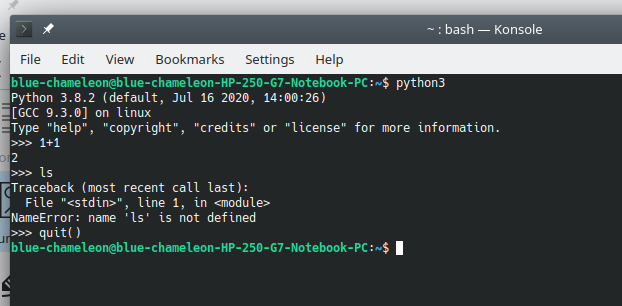
\includegraphics[width=\linewidth]{./gfx/interpreterConsole}
\end{minipage}
%
\end{frame}

% =========================================================================== %

\begin{frame}[fragile]{More Complex Codes: Script Files}
%
\vspace{-10pt}
%
\begin{minipage}[t]{.29\linewidth}
\vspace{0pt}
\begin{itemize}
\item Usually several hundred to thousands of lines of code
\item Impractical to type them again and again
\item[\Thus] Text file, holds all Python commands in sequence
\item Will be executed \emph{line by line}
\end{itemize}
\end{minipage}
%
\begin{minipage}[t]{.03\linewidth}
\phantom{lol}
\end{minipage}%
%
\begin{minipage}[t]{.65\linewidth}
\vspace{0pt}
\begin{codebox}[Code: \texttt{001-helloWorld.py}]
\begin{minted}[linenos, fontsize=\scriptsize]{python}
print("Hello World")
\end{minted}
\end{codebox}
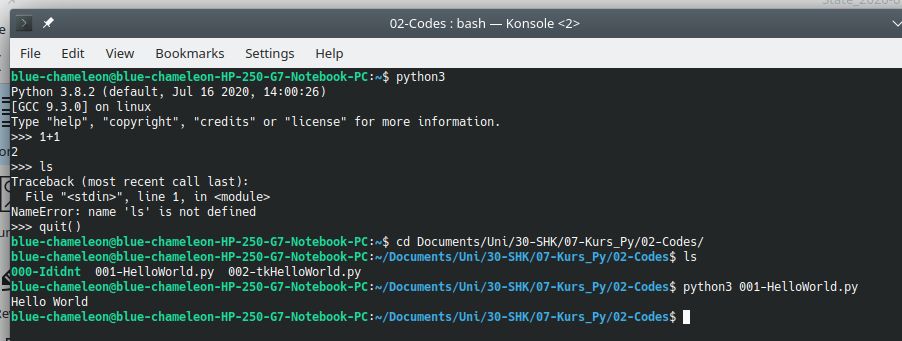
\includegraphics[width=\linewidth]{./gfx/print-HelloWorld-Run}
\end{minipage}
%
\end{frame}

% =========================================================================== %

\begin{frame}[fragile]{The IDE \emph{Spyder}}
%
\begin{center}
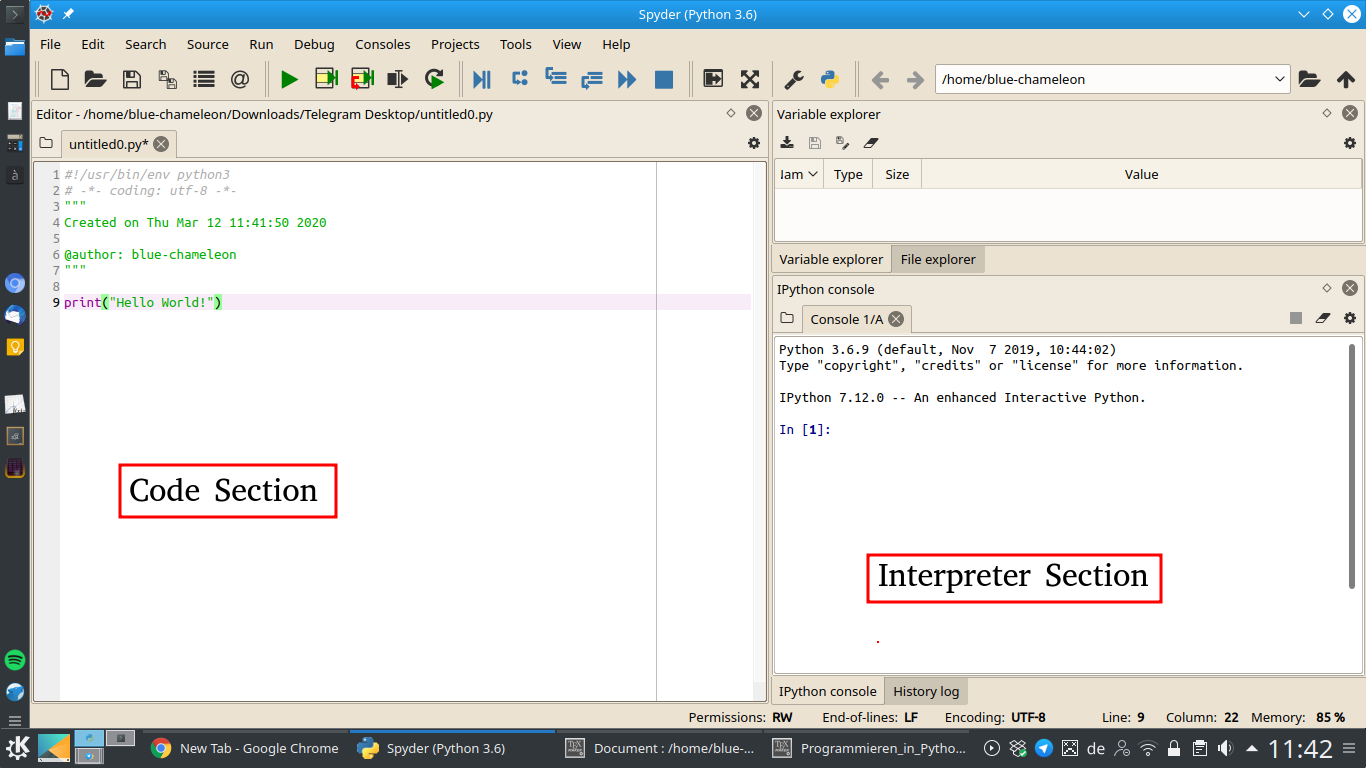
\includegraphics[width=.8\linewidth]{./gfx/Spyder}
\end{center}
%
\end{frame}

% =========================================================================== %

\begin{frame}[fragile]{The First Command: \inPy{print}}
%
\begin{itemize}
\item Causes output on screen
\item Necessary for working with script files
\item \emph{Parameters} in (parentheses)
\item Parameter: text(s) to be printed on screen, separated by commas
\item Texts encased by \texttt{'}single\texttt{'} or \texttt{''}double\texttt{''} quotes
\end{itemize}

\vspace{10pt}
\begin{minipage}{.49\linewidth}
\begin{codebox}[Code: \texttt{print}]
\begin{minted}[linenos, fontsize=\scriptsize]{python}
print("Text")
print('and even', "more text")
\end{minted}
\end{codebox}
%
\end{minipage}
\begin{minipage}{.49\linewidth}
\begin{cmdbox}[Output: \texttt{print}]
\begin{minted}[fontsize=\scriptsize]{text}
Text
and even more text
\end{minted}
\end{cmdbox}
\end{minipage}
\end{frame}

% =========================================================================== %

\begin{frame}{Error Messages}
%
\begin{minipage}[t]{.29\linewidth}
\begin{itemize}
\item Python reports file and line number when it finds an error
\item If input directly into terminal: \texttt{<stdin>, line 1}
\item Copy of the line that could not be translated
\end{itemize}
\end{minipage}
%
%
\begin{minipage}[t]{.69\linewidth}
\vspace{0pt}
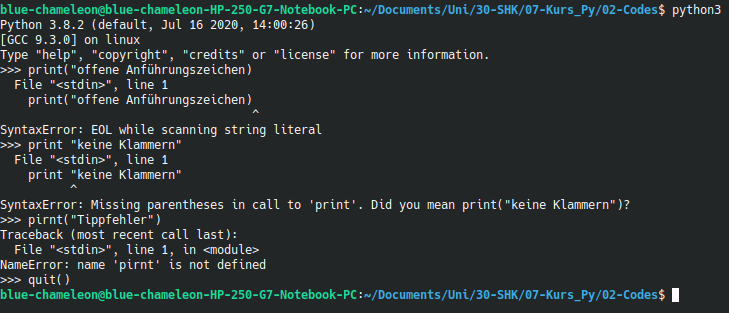
\includegraphics[width=\linewidth]{./gfx/errMsgs}
\end{minipage}
%

\vspace{6pt}
\begin{itemize}
\item Type of Error (SyntaxError, NameError, ...)
\end{itemize}
%
\end{frame}

% =========================================================================== %

\begin{frame}{Variables}
%
\begin{itemize}
\item Symols that store some value: \inPy{x = -7.5} or \inPy{x = "Wir Sind Helden"}
	\begin{itemize}
	\item \emph{Value}: Any sort of information: numbers, texts, pictures, entire programs, ...
	\end{itemize}
\item May be used in complex \emph{expressions}: \inPy{2 * (x + 7) * x}
	\begin{itemize}
	\item \emph{expression}: bit of code that can be \emph{evaluated} into a single value
	\end{itemize}
\item Can be overwritten: \inPy{x = x + 1}
\item Can be used with commands: \inPy{print(x)}
\item Can (and should!) comprise of several characters: \inPy{mouseCoordinate = 17}
\item Valid Characters: a-z, A-Z (case sensitive!), underscore (\_); 0-9 except for the first character
\item Recommendation: either \emph{Camel Case}: \inPy{mouseCoordinate}; or \emph{Snake Case}: \inPy{mouse_coordinate}
\item Technically possible but problematic: overwriting key words: \inPy{print = 3} \\
	(mark syntax highlighting of your IDE)
\end{itemize}
%
\end{frame}

% =========================================================================== %

\begin{frame}{Arithmetic Operators}
%
\newcolumntype{O}{>{\centering\ttfamily\arraybackslash}m{.1 \textwidth}}
\newcolumntype{F}{>{\centering         \arraybackslash}m{.6 \textwidth}}
\newcolumntype{X}{>{\centering\ttfamily\arraybackslash}m{.2 \textwidth}}
%
\rowcolors{1}{white}{tabhighlight}
%
\begin{tabularx}
	{\linewidth}
	{OFX}
	\toprule[1.5pt]

	\normalfont	\bfseries Symbol &
				\bfseries Function &
				\bfseries Example
	\tabcrlf
	+  & Addition                    & 1 + 2 = 3 \\
	-  & Subtraction                 & 5 - 7 = -2 \\
	*  & Multiplication              & 2 * 4 = 8 \\
	/  & Division                    & 7 / 5 = 1.4 \\
	// & Integer-Division            & 7 // 5 = 1 \\
	\% & Modulo (Rest of a Division) & 7 \% 5 = 2 \\
	** & Power                       & 3 ** 2 = 9 \\
	
	\bottomrule[1.5pt]	
\end{tabularx}
\begin{itemize}
\item Parentheses and order of operations is obeyed
\item Arbitrary number of nested parentheses
\end{itemize}
%
\end{frame}

% =========================================================================== %

\begin{frame}{Shorthands}
%
\begin{itemize}
\item Syntax element: \texttt{variable += expression}
\item Abbreviation for operations in the form of \inPy{variable = variable + expression}
\item Likewise: \inPy{-=}, \inPy{*=}, \inPy{/=}, ...
\item For the computer, both are translated the same way
\item But: removes a source of errors
	\begin{itemize}
	\item Code almost never is written top-to-bottom
	\item Insertations, trial-and-error, corrections
	\item Easy to forget updating both ends of the assignment statement
	\end{itemize}
\end{itemize}
%
\end{frame}

% =========================================================================== %

\begin{frame}[fragile]{Objects in Memory}
%
\begin{columns}
\column{.5\linewidth}
	\begin{itemize}
	\item \emph{All} objects: internally only numbers
	\item Example, letters (characters): 
		assignment number $\leftrightarrow$ glyph via table
	\item More complex objects: groups of numbers
	\item Example: picture: red-, green-, blue intensity of first pixel, second pixel, \ldots
	\item Only context tells how to interpret information
	\end{itemize}
\column{.5\linewidth}
	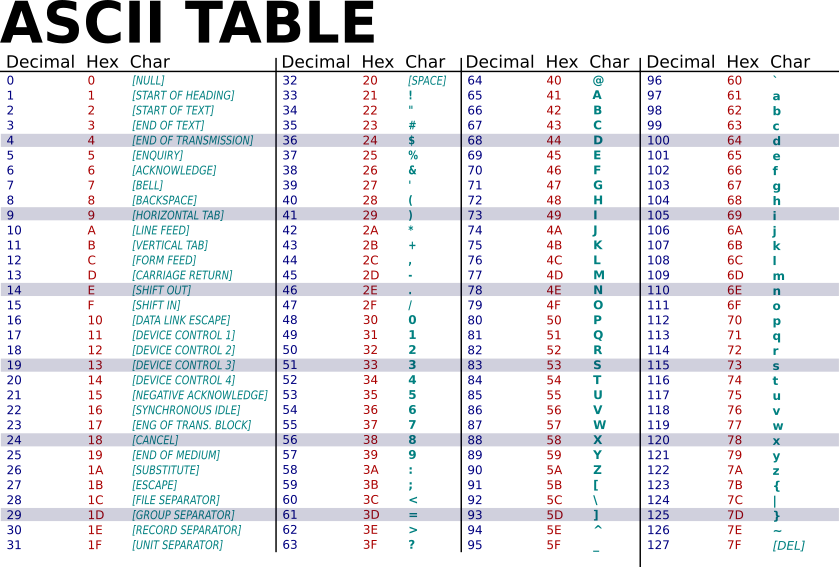
\includegraphics[width=\linewidth]{./gfx/ASCII_table}\newline
	\tiny ASCII: American Standard Code for Information Interchange\newline
	Quelle: \url{source: https://commons.wikimedia.org/wiki/File:ASCII-Table-wide.svg}
\end{columns}
%
\end{frame}

% =========================================================================== %

\begin{frame}{Data Types}
%
\begin{itemize}
\item Each expression (\zB variable) has assigned information: what is it?
\item This gives context for \enquote{computations}
\item Example: text vs. number:
	\begin{itemize}
	\item \inPy{"1" + "2"} \thus~ \inPy{"12"}
	\item \inPy{1 + 2} \thus~ \inPy{3}
	\end{itemize}
\item Data types:
	\begin{itemize}
	\item \inPy{int} -- integers (no decimal point)
	\item \inPy{float} -- \enquote{floating point numbers}, reals
	\item \inPy{complex} -- complex numbes: \inPy{z = 5.3 - 1j}
	\item \inPy{str} -- text (\enquote{string})
	\end{itemize}
\item Find out data type: \inPy{print(type(expression))}
\end{itemize}
%
\end{frame}

% =========================================================================== %

\begin{frame}[fragile]{Comments}
%
\begin{columns}[T]
\column{.5\linewidth}
\begin{itemize}
\item Line of text that will be ignored by the interpreter
\item Contains text for the develloper(s): explanations, etc.
\item Switching on and off a statement for testing purposes
\item Begin with a pound sign (\texttt{\#})
\item Entire line behind the pound sign will be ignored
\end{itemize}
%
\column{.5\linewidth}
\begin{codebox}[Code with comments]
\begin{minted}[linenos, fontsize=\scriptsize]{python}
print("Hello World")  # text output

# a comment may be a line of its own

# nested # comments do not exist

# print("this line will not be executed")
\end{minted}
\end{codebox}
\end{columns}
%
\end{frame}

\end{document}

% MAREI!!
% whom do I give credit? Where?